
%%%  یک نمونه پروپوزال کارشناسی ارشد، نسخه 0.4
%%%  وحید دامن‌افشان، دانشگاه تبریز،       http://www.damanafshan.ir
%%%   آپدیت شده در تیرماه ۹۱
%توضیحات مربوط به هر بسته یا دستور را می‌توانید در خط بالای آن ببینید.

\documentclass[12pt,a4paper]{article}
%در ورژن جدید زی‌پرشین برای تایپ متن‌های ریاضی، این سه بسته، حتماً باید فراخوانی شود
\usepackage{amsthm,amssymb,amsmath}

%دستوری برای وارد کردن واژه‌نامه انگلیسی به فارسی
\newcommand\persiangloss[2]{#1\dotfill\lr{#2}\\}
%بسته‌ای برای تنطیم حاشیه‌های بالا، پایین، چپ و راست صفحه
%\usepackage[top=30mm, bottom=30mm, left=30mm, right=30mm]{geometry}
%بسته‌ای برای نمایش تصاویر قرار داده شده در متن
\usepackage{graphicx}
% بسته‌ و دستوراتی برای ایجاد لینک‌های رنگی با امکان جهش
\usepackage[pagebackref=false,colorlinks,linkcolor=blue,citecolor=magenta]{hyperref}
% چنانچه قصد پرینت گرفتن نوشته خود را دارید، خط بالا را غیرفعال و  از دستور زیر استفاده کنید چون در صورت استفاده از دستور زیر‌‌، 
% لینک‌ها به رنگ سیاه ظاهر خواهند شد و برای پرینت گرفتن، مناسب‌تر خواهد بود.
%\usepackage[pagebackref=false]{hyperref}
%بسته‌ای برای ظاهر شدن «مراجع»  در فهرست مطالب
\usepackage{tocbibind}
%فراخوانی بسته زی‌پرشین و دستورات مربوط به نوع فونت‌ها
\usepackage{xepersian}
%تغییرات نخ
\usepackage[bottom]{footmisc}
\usepackage{indentfirst}


\settextfont{B Nazanin}
% وارد کردن دستور بالا الزامی نیست؛ چون در صورت وارد نکردن آن، فونت پیش‌فرض به صورت خودکار، فراخوانی می‌شود.
% چنانچه می‌خواهید که اعداد داخل فرمول‌ها، فارسی باشد، دستور زیر را فعال کنید
%\setdigitfont{Times New Roman}


%%%%%%%%%%%%%%%%%%%%%%%%%%%%%%%%%%%%%%%%%%%%%%%%%%%
% تعریف قلم‌های فارسی و انگلیسی برای استفاده در بعضی از قسمت‌های متن
\defpersianfont\titr[Scale=1]{B Titr}
\defpersianfont\nastaliq[Scale=1.5]{IranNastaliq}
\defpersianfont\traffic[Scale=1]{B Traffic}
\defpersianfont\yekan[Scale=1]{B Yekan}
\DefaultMathsDigits
%اگر فونت‌های بالا را ندارید، دو خط بالا را غیر فعال و دو خط زیر را فعال کنید
%\defpersianfont\traffic[Scale=1]{XB Roya}
%\defpersianfont\yekan[Scale=1]{XB Kayhan}
%%%%%%%%%%%%%%%%%%%%%%%%%%%%%%%%%%%%%%%%%%%%%%%%%%%
% تعریف و نحوه ظاهر شدن قضایا، لم‌ها، تعریف‌ها و ...
\theoremstyle{definition}
\newtheorem{definition}{تعریف}[section]
\theoremstyle{theorem}
\newtheorem{theorem}[definition]{قضیه}
\newtheorem{lemma}[definition]{لم}
\newtheorem{proposition}[definition]{گزاره}
\newtheorem{corollary}[definition]{نتیجه}
\newtheorem{remark}[definition]{ملاحظه}
\theoremstyle{definition}
\newtheorem{example}[definition]{مثال}
%%%%%%%%%%%%%%%%%%%%%%%%%%%%%%%%%%%%%%%%%%%%%%%%%%%
\begin{document}
% دستوری جهت حذف کردن شماره صفحه و سربرگ، در صورت وجود (فقط در صفحه جاری)
\thispagestyle{empty}
\vspace*{-28mm}
% نحوه درج کردن لوگوی دانشگاه
\centerline{
\includegraphics[height=5cm]{logo.jpg}}
\begin{center}
%دستوری برای کم کردن فاصله بین لوگو و خط پایین آن
\vspace{-2mm}
{\large \titr
گروه مستقل مهندسی رباتیک
%دستوری برای تعیین فاصله بین دو خط
\\[2.1cm]
}

{\Large \titr
تمرین اول درس بینایی ماشین
\\[2cm]
استاد درس:
\\[.5cm]
دکتر صفابخش
\\[1.5cm]
\large 
تدریس‌یار: 
\\[0.5cm]
مهندس مجد
\\[1.5cm]
نام دانشجو:
\\[.5cm]
نوید خزاعی
\\[.5cm]
۹۲۱۳۵۰۰۸
\\[1.5cm]
}
%دستوری برای تعیین فاصله بین خطوط (نه دو خط) و تا وقتی که مقدار آن تغییر نکند، فاصله بین خطوط، همین مقدار است.
\baselineskip=1cm

{\large
زمستان ۱۳۹۲
}
\end{center}
%دستوری برای رفتن به صفحه جدید
\newpage
\baselineskip=1cm
%دستوری برای ظاهر شدن فهرست مطالب
\tableofcontents

\baselineskip=.75cm
\newpage 
\section{بخش اول}
%\cite{alvarez}
\subsection{{\lr {Normalization - ‫‪Contrast‬‬ ‫‪Stretching‬‬}
}
}



\textbf{پرسش:}
عملگر 
\lr {Contrast Stretching}
یا 
\lr {Normalization}
چیست؟ برای تصویر شماره‌ی ۱ این عملگر را اعمال کنید. عملگر چه تاثیری داشته است؟

\textbf{پاسخ:}
عملگر 
\lr{Contrast Stretching}
یا
\lr{Normalization}
، عملگری است که استفاده از آن سبب می‌شود پیکسل‌ها بازه‌های بیشتری از رنگ‌های موجود را پوشش بدهند و سبب می‌شود کنتراست بین ویژگی‌ها و پس‌زمینه‌ی آن‌ها زیاد شود. این عملگر دو نوع خطی و غیر خطی دارد. در نوع خطی،‌ دو مقدار مرزی بالایی و پایینی (معمولا کمینه و بیشینه مقادیر روشنایی موجود در تصویر) استفاده می‌شوند تا طی تبدیل زیر\LTRfootnote{\vspace{0.1cm}
 http://en.wikipedia.org/wiki/Normalization\_\%28image\_processing\%29
}، مقادیر هیستوگرام را
\lr{Stretch}
کنند (بِکِشند) تا تمام مقادیر ممکن برای روشنایی پوشش داده‌شود. 
\\

\vspace{0.3cm}
\begin{equation}
\label{linear}
I_N = (I - Min ) {{newMax - newMin} \over {Max - Min}} + newMin
\end{equation}


\centerline{\vspace{-1cm} 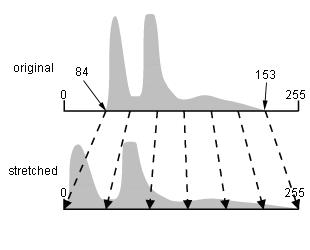
\includegraphics[height=7cm]{linearstretch.jpg}}
\centerline{\vspace{0.6cm}
شکل ۱ - تبدیل خطی
\LTRfootnote{ http://hosting.soonet.ca/eliris/remotesensing/LectureImages/linearstretch.gif
}
}
در نسخه‌ی غیرخطی، که به
\lr{Equalized Contrast Stretch}
نیز معروف است، مقادیر روشنایی بیشتری (بازه‌ی بیشتری از هیستوگرام) به بخش‌هایی که بیشتر در هیستوگرام ظاهر شده‌اند، نسبت داده می‌شود. 
\\ 

\centerline{\vspace{-0.5cm} 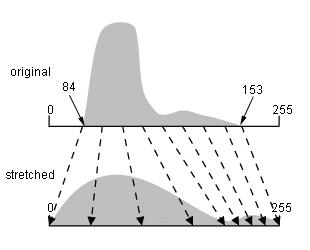
\includegraphics[height=7cm]{equalizedstretch.jpg}}
\centerline{\vspace{0.6cm}
شکل ۲ - تبدیل غیر خطی
\LTRfootnote{ http://hosting.soonet.ca/eliris/remotesensing/LectureImages/equalizedstretch.gif
}
}
برای اعمال این عملگر به تصویر، از تابع

\leftline {\lr{normalize(\_src, dst, 0, 255, NORM\_MINMAX, CV\_8UC1)}}

 استفاده نمودیم که در آن مقادیر 
\(newMax\)
و 
\(newMin\)
به ترتیب برابر با 
\lr0
و 
\lr{255}
انتخاب شده‌اند تا تمامی مقادیر پوشش یابند. با استفاده از 
\lr{NORM\_MINMAX}
، نرمال‌سازی با روش خطی و با به‌دست آوردن کمینه و بیشینه‌ی تصویر انجام می‌شود.
دلیل استفاده از
\lr{CV\_8UC1}
نیز، استفاده از عکس خاکستری با بازه‌ی 
\lr{(0,255)}
است (نمایش هشت بیتی و تک کاناله).


نتایج اعمال این عملگر بر روی تصویر شماره‌ی ۱ در زیر آورده شده‌است. همان‌گونه که مشاهده می‌کنید، مقادیر خاکستری بیشتری به تصویر اختصاص داده شده‌است و اختلاف مقادیر خاکستری نزدیک به هم، بیشتر و در نتیجه کنتراست، بهتر شده‌است.
\vspace{0.1cm}

\begin{center}
\begin{tabular}{@{}cc@{}}
\frame{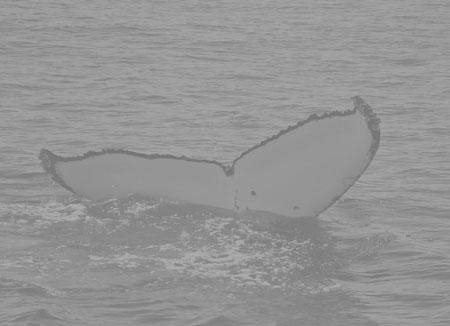
\includegraphics[height=40mm]{1.jpg}}&
\frame{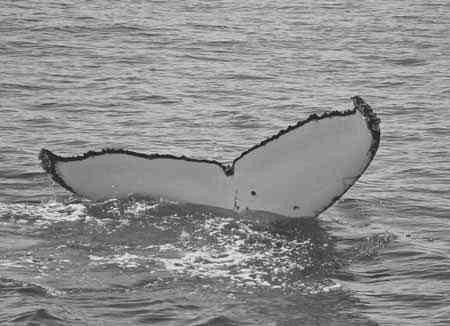
\includegraphics[height=40mm]{1-p.jpg}} \\ 
\small \textbf{قبل از نرمال‌سازی} & \small \textbf{پس از نرمال‌سازی}
\end{tabular}
\vspace{1cm}
\end{center}
\subsection{تاثیر نرمال‌سازی}
\textbf{پرسش: }
این عملگر در چه تصاویری تغییر ایجاد کرده و برای کدام تصاویر بی‌اثر است؟ نمونه‌ای از تصویری که این عملگر بر روی آن بی‌اثر است تهیه کرده و نتیجه را تحلیل کنید.


\textbf{پاسخ: } 
با بسط فرمول 
\eqref{linear}
خواهیم داشت: 
\begin{equation}
\DeclareMathSizes{8}{16}{10}{6}
\textstyle
\label{nkhLinear}
I_N = I \left( {{newMax - newMin} \over {Max - Min}} \right) - Min \left( {{{newMax - newMin} \over {Max - Min}} } \right) + newMin
\end{equation}
برای آن‌که 
\( I_N = I \)
، باید عبارت 
\( {{newMax - newMin} \over {Max - Min}}  \)
برابر با یک باشد و حاصل ترم‌های باقی‌مانده صفر شود. پس کافی است که 
\( newMin = Min \)
 و 
 \( newMax = Max \)
 باشد. به دیگر سخن،‌ نرمال‌سازی خطی هر تصویر، با انتخاب بازه‌ی 
 \lr{Stretch}
 تعریف شده با کمینه و بیشینه‌ی تصویر، بی‌اثر خواهد بود. برای نمونه، تصویری که مقادیر \lr0 و \lr{255} را در خود دارد، با تابع \lr{normalize} و آرگومان‌های آورده‌شده‌ (\lr{\(newMin=0 , newMax=255\)}
)، تغییری نخواهد کرد. برای اثبات این ادعا، از همان تصویر قبلی استفاده کردیم. به این ترتیب که دو ناحیه‌ی کوچک سفید و سیاه به تصویر اضافه نمودیم که با دوایر قرمز رنگ مشخص شده‌اند. نتیجه را در زیر مشاهده می‌فرمایید:
\begin{center}
\vspace{5mm}
\begin{tabular}{@{}cc@{}}
\frame{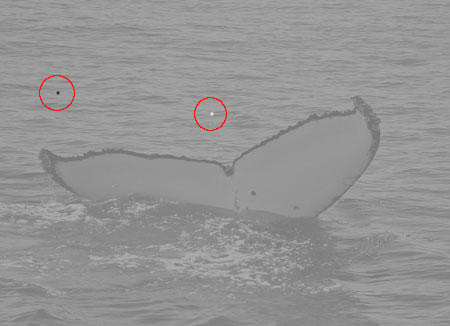
\includegraphics[height=40mm]{11-c.jpg}} &
\frame{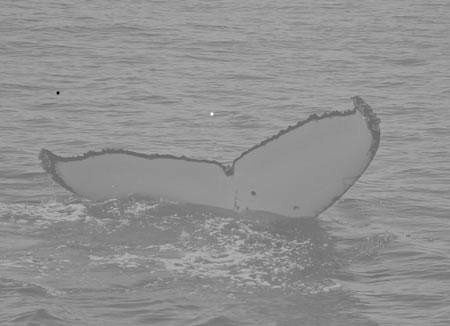
\includegraphics[height=40mm]{11-p.jpg}} \\ 
\small \textbf{قبل از نرمال‌سازی} & \small \textbf{پس از نرمال‌سازی}
\end{tabular}
\vspace{0.5cm}
\end{center} 

\subsection{\lr{Histogram Equalization}}

\textbf{پرسش: }
\lr{Histogram Equalization}
چیست؟ برای تصویر شماره‌ی ۱ این عملگر را اعمال کنید. عملگر چه تاثیری داشته‌است؟ 


\textbf{پاسخ: } 
تعدیل هیستوگرام، عملی است که طی آن هیستوگرام را به گونه‌ای تغییر می‌دهیم که تمرکز نقاط از روی مقادیر معین در هیستوگرام، از بین برود و بازه‌ی مقادیر استفاده‌شده در هیستوگرام، بیشتر شود. به دیگر سخن، از هر مقدار خاکستری، تعداد مناسبی در تصویر خواهیم داشت و شکل ظاهری هیستوگرام، تعدیل می‌شود. 

برای این منظور، اگر تصویر با ابعاد 
\lr{\(N \times N\)}
را در نظر بگیریم، که 
\lr{\(L\)} 
سطح خاکستری دارد و برای هر نقطه، مقدار سطح خاکستری برابر با 
\lr{\(r_k\)}
باشد و 
\lr{\(r_k \in \lbrace 0,1,...,L-1 \rbrace \)}
، اگر تعداد نقاطی که سطح خاکستری
\lr{\(r_k\)}
دارند، 
\lr{\(n_k\)}
آن‌گاه خواهیم داشت: 
\lr{
\[ p(r_k) = { {n_k} \over {N^2} } \phantom{ba}, \phantom{ba} k=0,1,...,L-1 \]
}
هدف به دست آوردن تابع تبدیل \( T\) است به گونه‌ای که با اعمال آن بر روی نقطه‌ای با سطح روشنایی \(p_j\) از تصویر اصلی، سطح روشنایی \(q_j\) برای آن نقطه در تصویر جدید را به‌دست دهد، که هیستوگرام حاصل از آن، مسطح باشد. به دیگر سخن، مقادیر روشنایی این‌بار از یک تابع چگالی یکنواخت پیروی خواهند کرد. همان‌گونه که در اسلاید‌های درس اشاره شده‌است، می‌توان نشان داد که این تابع تبدیل به صورت زیر است:
\vspace{0.2cm}
\begin{equation}
\label{histeq}
 q_j = T(p_j) = {{q_k - q_0} \over {N^2} } \sum_{i=p_0}^{p_j}{G(i)+q_0} 
\end{equation}
که در آن \(G\) هیستوگرام تصویر اصلی است.

در \lr{OpenCV} از تابع زیر برای تعدیل هیستوگرام استفاده می‌شود:

\leftline{\lr{equalizeHist(src,dst)}}

که نتیجه‌ی اعمال آن بر روی تصویر ۱، به این شکل است:

\begin{center}
\vspace{5mm}
\begin{tabular}{@{}cc@{}}
\frame{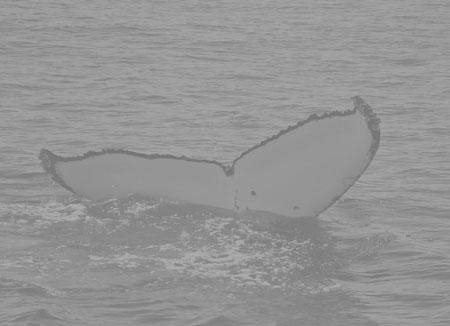
\includegraphics[height=40mm]{1.jpg}} &
\frame{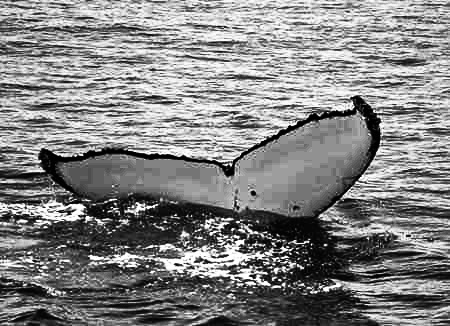
\includegraphics[height=40mm]{1-eq.jpg}} \\ 
\small \textbf{قبل از تعدیل} & \small \textbf{پس از تعدیل}
\end{tabular}
\vspace{0.5cm}
\end{center} 
\vspace{0.5cm}
همان‌گونه که مشاهده می‌فرمایید، این عملگر، کنتراست تصویر یا به دیگر سخن، وضوح آن‌ را، بیشتر می‌کند. این در نتیجه‌ی تنوع سطوح خاکستری و تعدیل تعداد نقاط از هر رنگ خاکستری است.
\vspace{0.5cm}
\subsection{مقایسه‬}

\textbf{پرسش:}
تفاوت دو عملگر فوق،
\lr{Contrast Stretching}
و
\lr{Histogram Equalization}
 در چیست؟ از نظر کارایی و سرعت با هم مقایسه کنید.

\textbf{پاسخ:}
یکی از تفاوت‌های اصلی، خطی بودن 
\lr{Contrast Stretching}
و غیر خطی بودن 
\lr{Histogram Equalization}
است. در عملگرِ اول، تفاوت ایجاد شده در تصویر، گاه بسیار اندک است اما حالت طبیعی تصویر حفظ می‌شود. برخلاف آن، عملگر تعدیل وضوح تصویر را بسیار بیشتر می‌کند اما به طور معمول تصویر را مصنوعی جلوه می‌دهد. 
از نظر سرعت، با توجه به فرمول‌های \eqref{linear} و \eqref{histeq}، به آسانی در‌می‌یابیم برای پیاده‌سازی \eqref{histeq}، یک حلقه‌ی اضافه برای محاسبه‌ی \( \sum \) نیاز داریم که یک مرتبه به مرتبه‌ی پیچیدگی اجرای الگوریتم بر روی تصویر، اضافه می‌کند. پس نرمال‌سازی خطی، به طور کلی، سریع‌تر از تعدیل هیستوگرام است. 

\subsection{رسم و مقایسه‌ی هیستوگرام}
\textbf{پرسش:}
هیستوگرام حاصل از اعمال
\lr{Contrast Stretching}
و
\lr{Histogram Equalization}
را بر روی یک تصویر با هم مقایسه کنید.

\textbf{پاسخ:}
برای این بخش از تصویر زیر استفاده نمودیم:
\vspace{0.15cm}

\begin{center}
\begin{tabular}{@{}cc@{}}
\frame{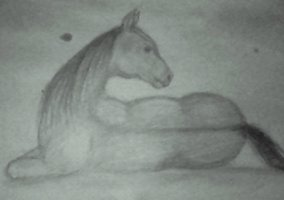
\includegraphics[height=4cm]{33.jpg}} &
\frame{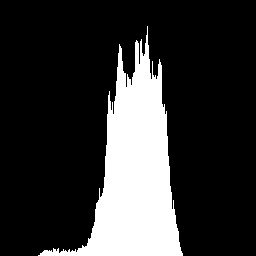
\includegraphics[height=40mm]{orig-showHist.jpg}} \vspace{0.25cm} \\ 

\small \textbf{ شکل ۳ - نقاشی اسب}\footnotemark & \small \textbf{ هیستوگرام شکل ۳} \vspace{0.5cm} \\ 
\frame{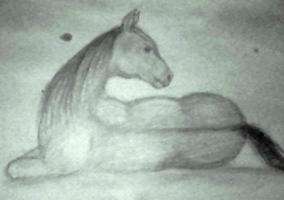
\includegraphics[height=4cm]{33-normalHist.jpg}} &
\frame{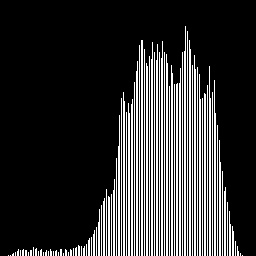
\includegraphics[height=40mm]{normal-showHist.jpg}} \vspace{0.25cm} \\ 

\small \textbf{ پس از نرمال‌سازی} & \small \textbf{ هیستوگرام نرمال} \\

\end{tabular}
\vspace{0.5cm}

\end{center} 
\LTRfootnotetext{ http://th01.deviantart.net/fs71/200H/f/2011/354/3/8/\\ \phantom{someSpace}another\_horse\_of\_bad\_quality\_by\_vulpes\_corsac-d4jplkf.png
}
\begin{center}
\begin{tabular}{@{}cc@{}}
 
\frame{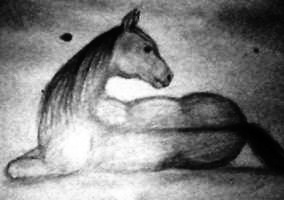
\includegraphics[height=4cm]{33-equalHist.jpg}} &
\frame{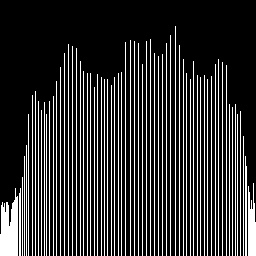
\includegraphics[height=40mm]{equal-showHist.jpg}} \vspace{0.25cm} \\ 

\small \textbf{ پس از تعدیل} & \small \textbf{ هیستوگرام تعدیل‌شده} \\

\end{tabular}
\vspace{0.5cm}

\end{center} 

همان‌گونه که مشاهده می‌فرمایید، عمل نرمال‌سازی تنها با کشیدن هیستوگرام به سمت دو سر انتهایی بازه، تلاش در بهبود تصویر دارد، اما تعدیل سبب شده است هیستوگرام مسطح‌تر شود و توزیع روشنایی نقاط، یکنواخت شود.

\section{ بخش ۲} 
\subsection{فیلترهای میانه، میانگین، گاوسی}

\textbf{پرسش:}
تفاوت فیلترهای میانه، میانگین و گاوسی در چیست؟ تصویری را نویزی کرده و هر سه فیلتر را به آن اعمال کنید. در سوالات این بخش شدت نویز را به گونه‌ای تنظیم کنید که تاثیر فیلترها قابل مشاهده باشد.

\textbf{پاسخ:}
تفاوت این فیلترها در شکل کلیشه‌ی به کار رفته در آن‌هاست که در هر کدام از منطق خاصی پیروی می‌کند و پیامدهای گوناگونی دارد. 

\begin{itemize}
\renewcommand{\labelitemi}{$\bullet$}
\item در فیلتر میانگین، میانگین شدت روشنایی نقاط همسایه، جایگزین شدت روشنایی نقطه‌ی کنونی می‌شود. به همین دلیل، جزییات تصویر حذف می‌شوند. این عمل، وضوح تصویر را هم کمتر می‌کند.
\item در فیلتر گاوسی، یک میان‌گیری وزن‌دار انجام می‌دهیم که وزن‌ها از توزیع گاوسی پیروی می‌کنند.  این فیلتر از فیلتر میانگین بهتر است.
\item در فیلتر میانه، همه‌ی همسایگی‌ها مرتب می‌شوند و میانه‌ی آن‌ها انتخاب می‌شود. به همین دلیل، می‌توان بر خلاف فیلترهای قبلی، چندین بار آن را به تصویر اعمال کرد. این فیلتر لبه‌های نازک را نیز از بین نمی‌برد و در کل عملکرد بهتری از دو فیلتر دیگر دارد. این فیلتر با کلیشه‌های صلیبی شکل نیز استفاده می‌شود.
برای آزمایش از فیلترهای ۳ \( \times \) ۳ و شکل ۴، استفاده نمودیم:


\begin{center}
\begin{tabular}{@{}cc@{}}
\frame{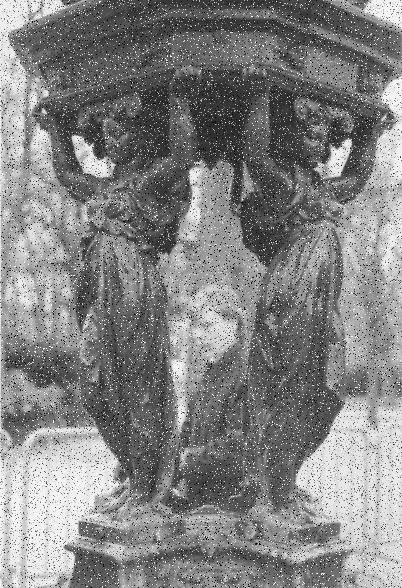
\includegraphics[height=7.5cm]{noise0.jpg}} &
\frame{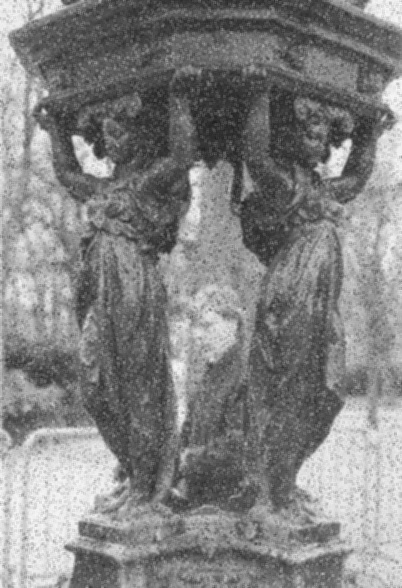
\includegraphics[height=7.5cm]{noise0-meaqnFilter.jpg}} \vspace{0.25cm} \\ 

\small \textbf{ شکل ۴ }\footnotemark & \small \textbf{ اعمال فیلتر میانگین} \vspace{0.5cm} \\ 
\frame{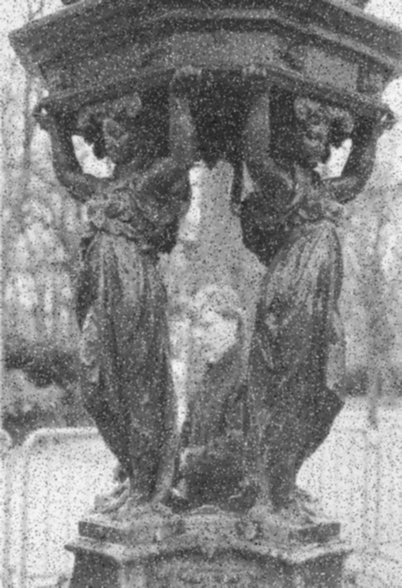
\includegraphics[height=7.5cm]{noise0-gaussionFilter.jpg}} &
\frame{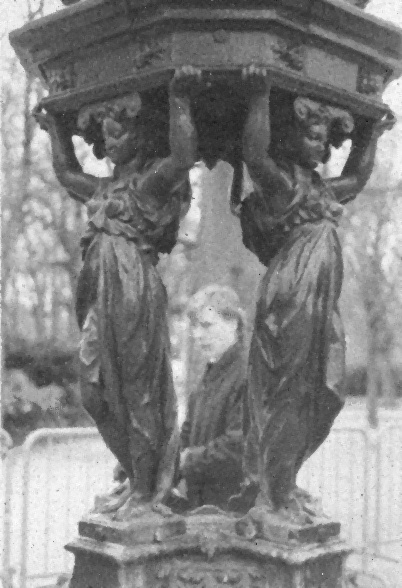
\includegraphics[height=7.5cm]{noise0-medianFilter.jpg}} \vspace{0.25cm} \\ 

\small \textbf{ اعمال فیلتر گاوسی} & \small \textbf{ اعمال فیلتر میانه} \\

\end{tabular}
\vspace{0.5cm}

\end{center} 
\LTRfootnotetext{ http://homepages.inf.ed.ac.uk/rbf/HIPR2/images/sta2noi1.gif
}

\end{itemize}
\vspace{0.2cm}

\subsection{اثر میانگین و میانه}

\textbf{پرسش:}
اثر دو فیلتر میانه و میانگین را بر نویزهای گاوسی، نمک‌فلفلی و یکنواخت مقایسه کنید. برای این‌کار تصویری را هر بار با یکی از نویزها آغشته کرده و سپس هر دو فیلتر را اعمال کنید. کدام‌یک در حذف نویز گوسی بهتر عمل می‌کنند؟ چرا؟

\textbf{پاسخ:}
میانگین بهتر نویز گاوسی را حذف می‌کند. چون خود نویز گاوسی شبیه نوعی میانگین وزن‌دار است.
نتایج به این شکل است:

\begin{center}
\makebox[\textwidth]{%
\begin{tabular}{@{}cc@{}}
\frame{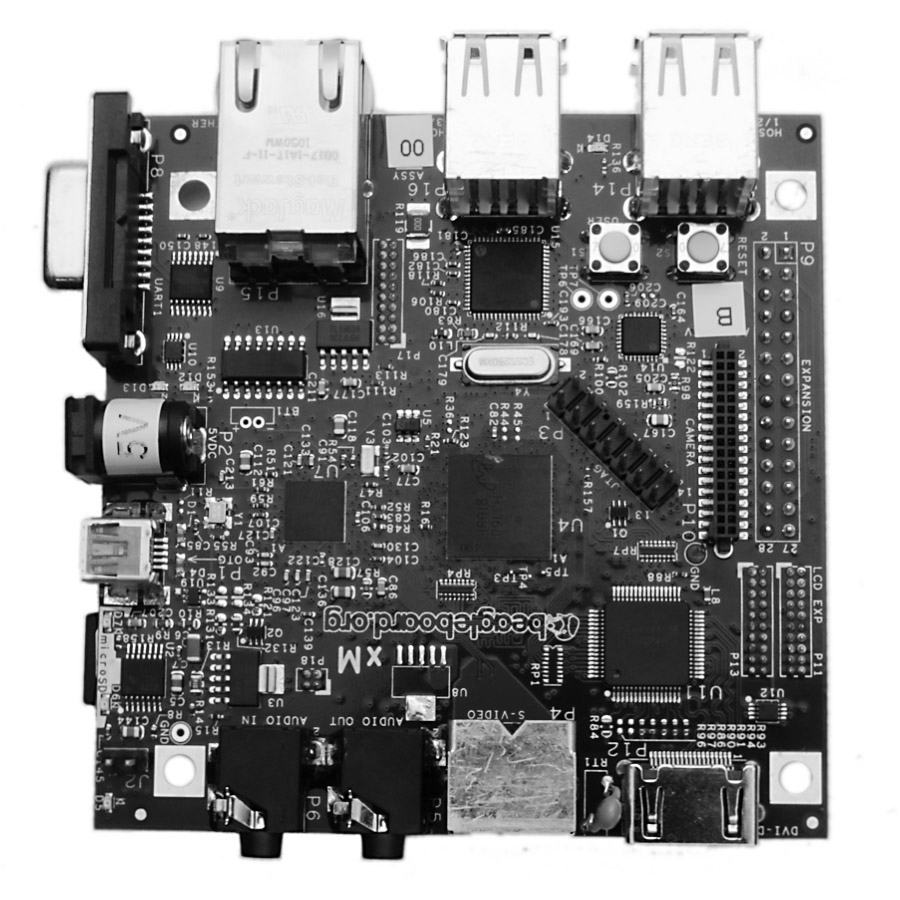
\includegraphics[height=7.5cm]{noise_tester.jpg}} &
\frame{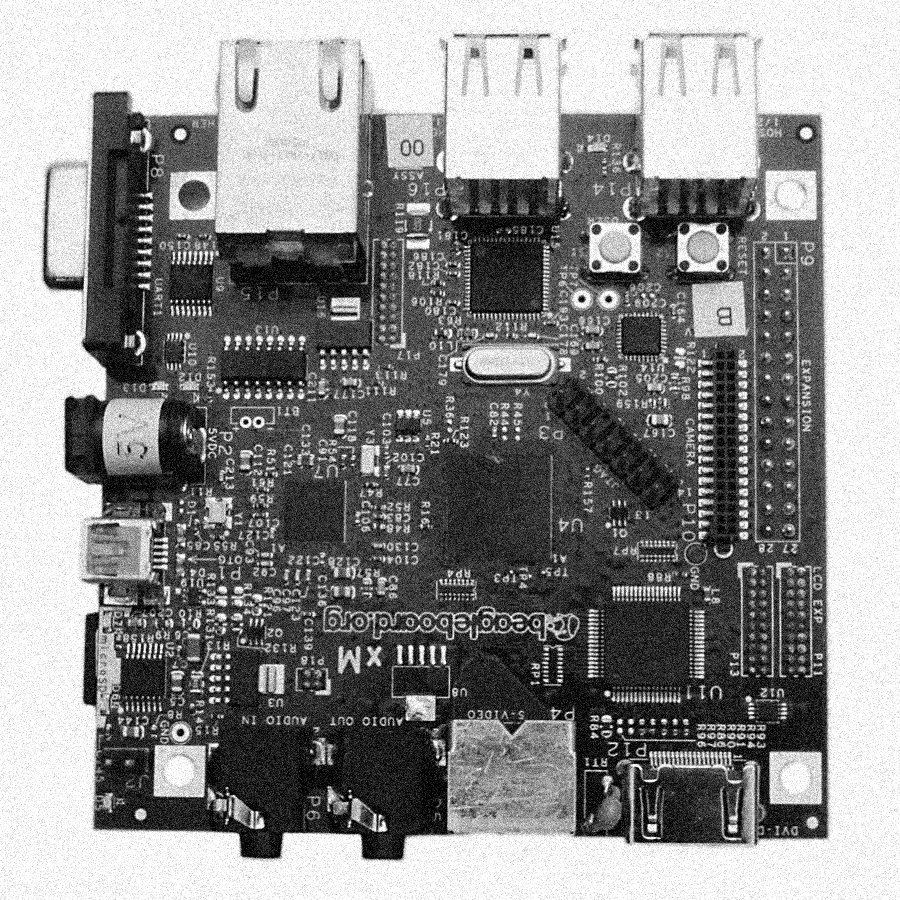
\includegraphics[height=7.5cm]{noise3-g.jpg}} \vspace{0.25cm} \\ 

\small \textbf{ شکل ۵ }\footnotemark & \small \textbf{ اعمال نویز گاوسی} \vspace{0.5cm} \\ 

\end{tabular}}
\vspace{0.5cm}
\end{center} 
\LTRfootnotetext{ http://www.liquidware.com/system/0000/3815/BeagleBoard\_xM\_Top.jpg
}


\begin{center}
\makebox[\textwidth]{%
\begin{tabular}{@{}cc@{}}
\frame{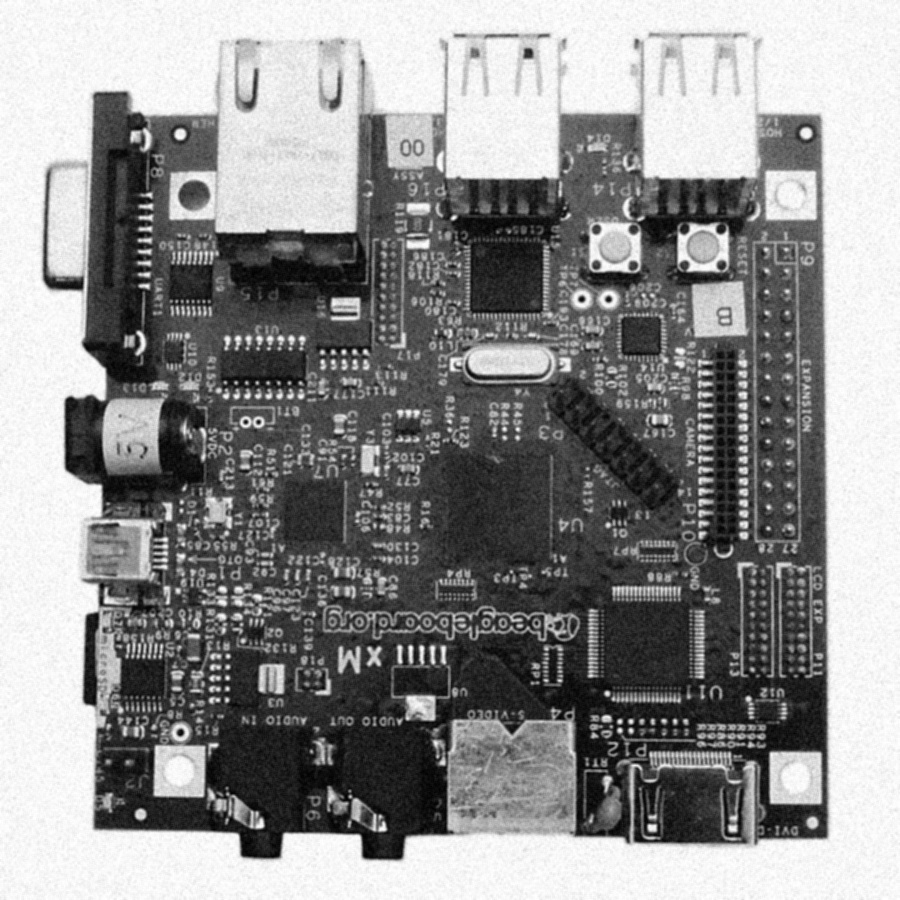
\includegraphics[height=7.5cm]{noise3-g-meaqnFilter.jpg}} &
\frame{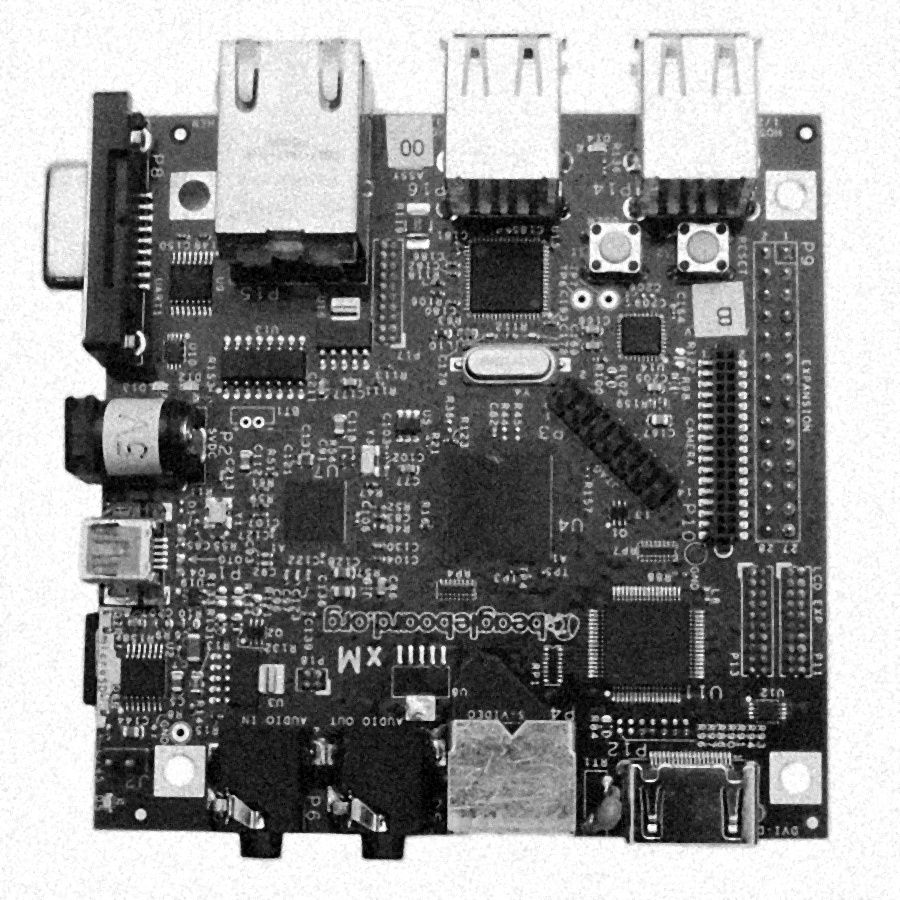
\includegraphics[height=7.5cm]{noise3-g-medianFilter.jpg}} \vspace{0.25cm} \\ 

\small \textbf{ اعمال فیلتر میانگین} & \small \textbf{ اعمال فیلتر میانه} \\

\end{tabular}}
\vspace{0.5cm}
\end{center} 

\begin{center}
\makebox[\textwidth]{%
\begin{tabular}{@{}cc@{}}
\frame{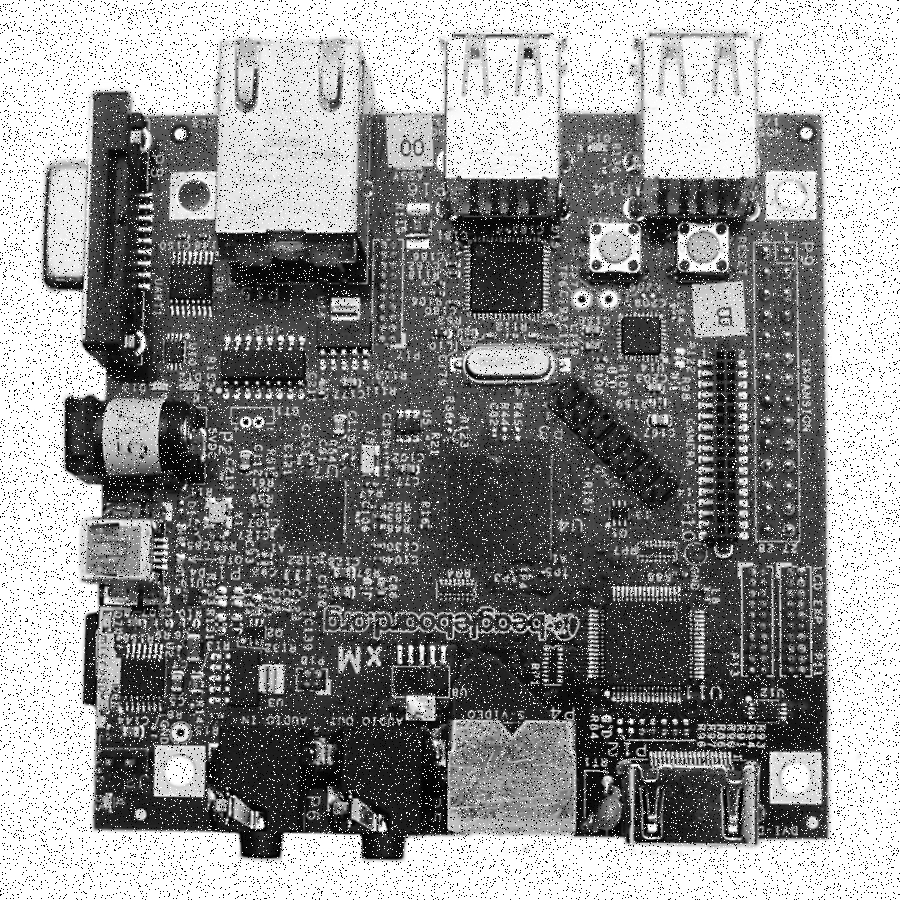
\includegraphics[height=7.5cm]{noise4-sult.jpg}} &
\frame{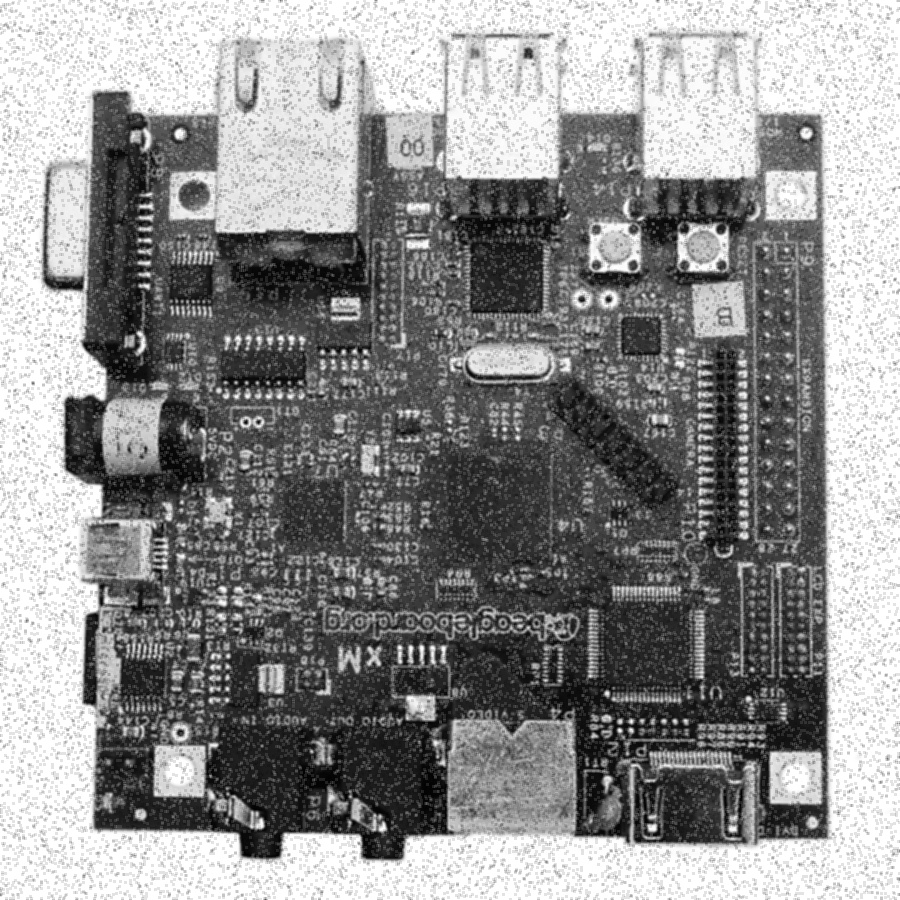
\includegraphics[height=7.5cm]{noise4-sult-meaqnFilter.jpg}} \vspace{0.25cm} \\ 

\small \textbf{ اعمال نویز نمک‌فلفلی } & \small \textbf{ اعمال فیلتر میانگین } \vspace{0.5cm} \\ 
\end{tabular}}
\vspace{0.5cm}
\end{center} 


\begin{center}
\makebox[\textwidth]{%
\begin{tabular}{@{}cc@{}}
\frame{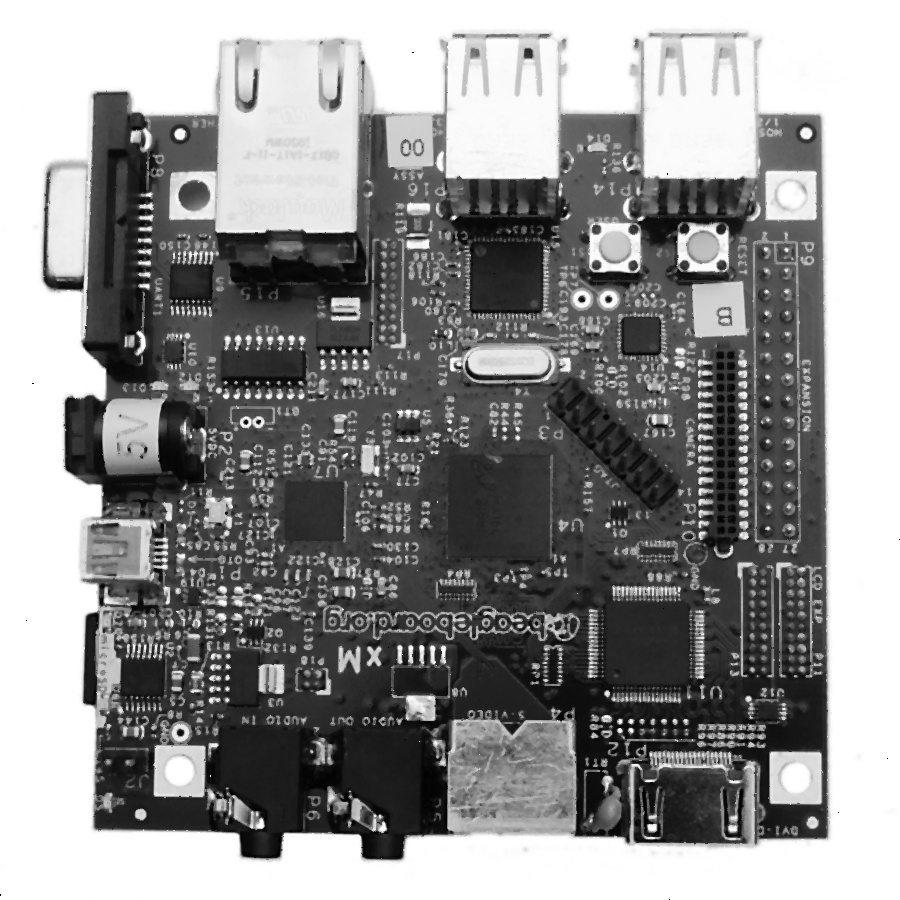
\includegraphics[height=7.5cm]{noise4-sult-medianFilter.jpg}} &
\frame{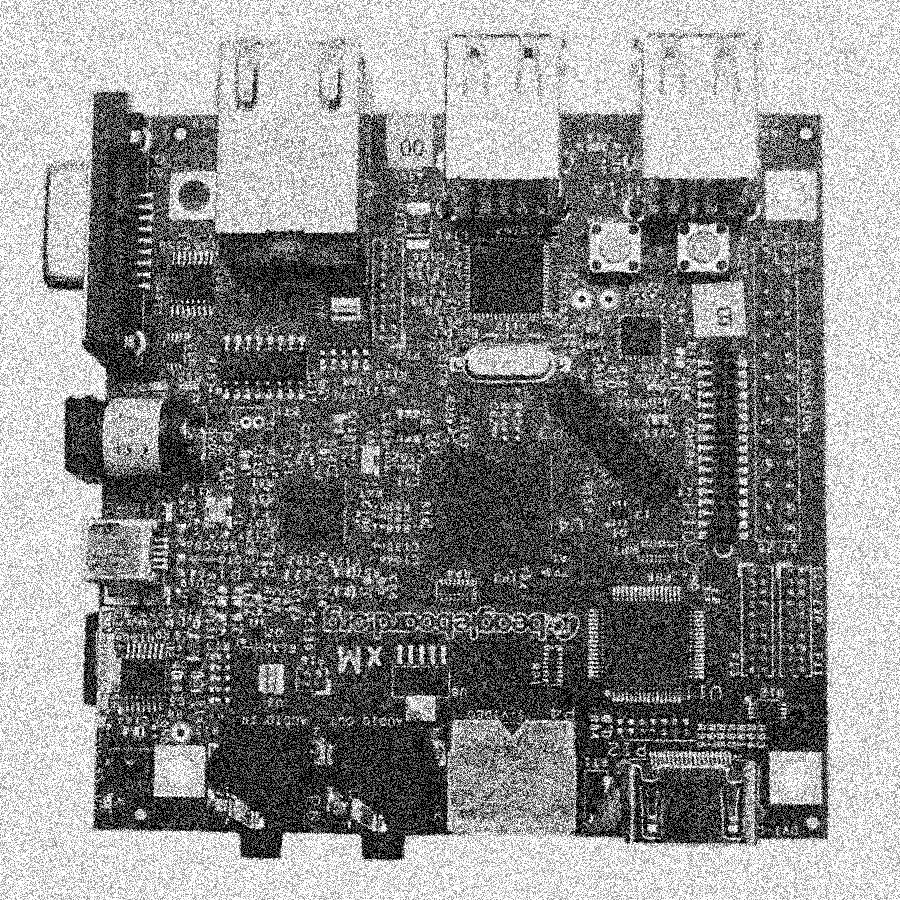
\includegraphics[height=7.5cm]{uniform.jpg}} \vspace{0.25cm} \\ 

\small \textbf{ اعمال فیلتر میانه} & \small \textbf{ اعمال نویز یکنواخت} \\
\end{tabular}}
\vspace{0.5cm}
\end{center} 

\begin{center}
\makebox[\textwidth]{%
\begin{tabular}{@{}cc@{}}
\frame{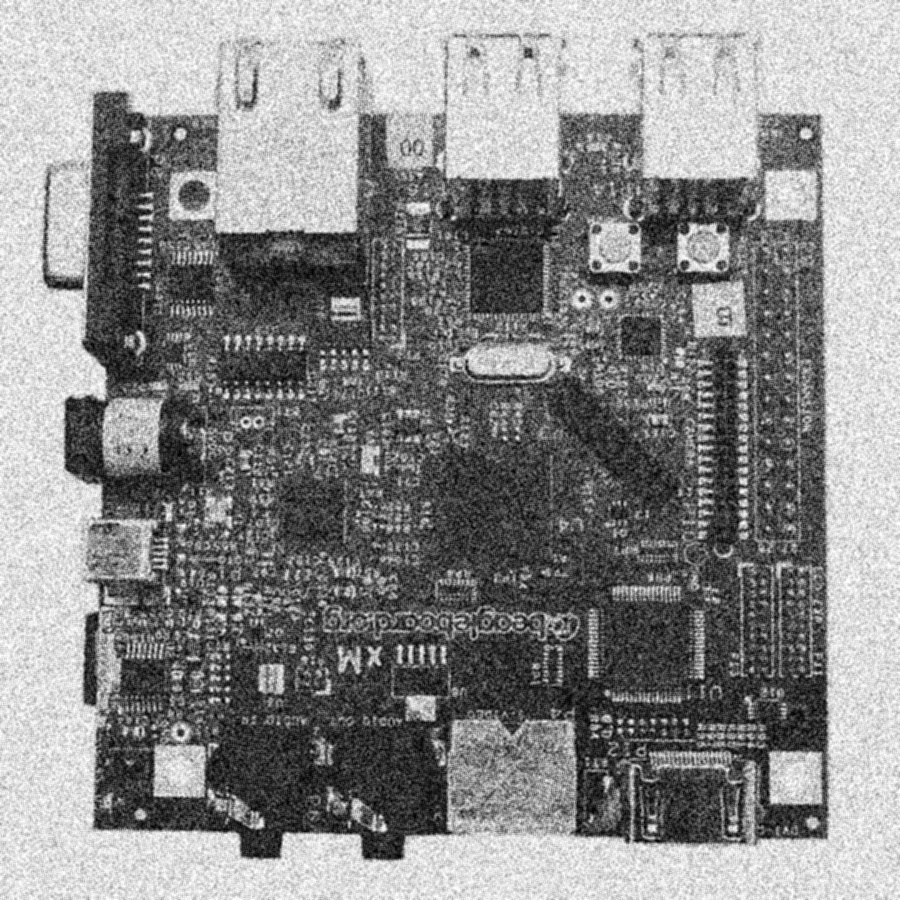
\includegraphics[height=7.5cm]{uniform-meaqnFilter.jpg}} &
\frame{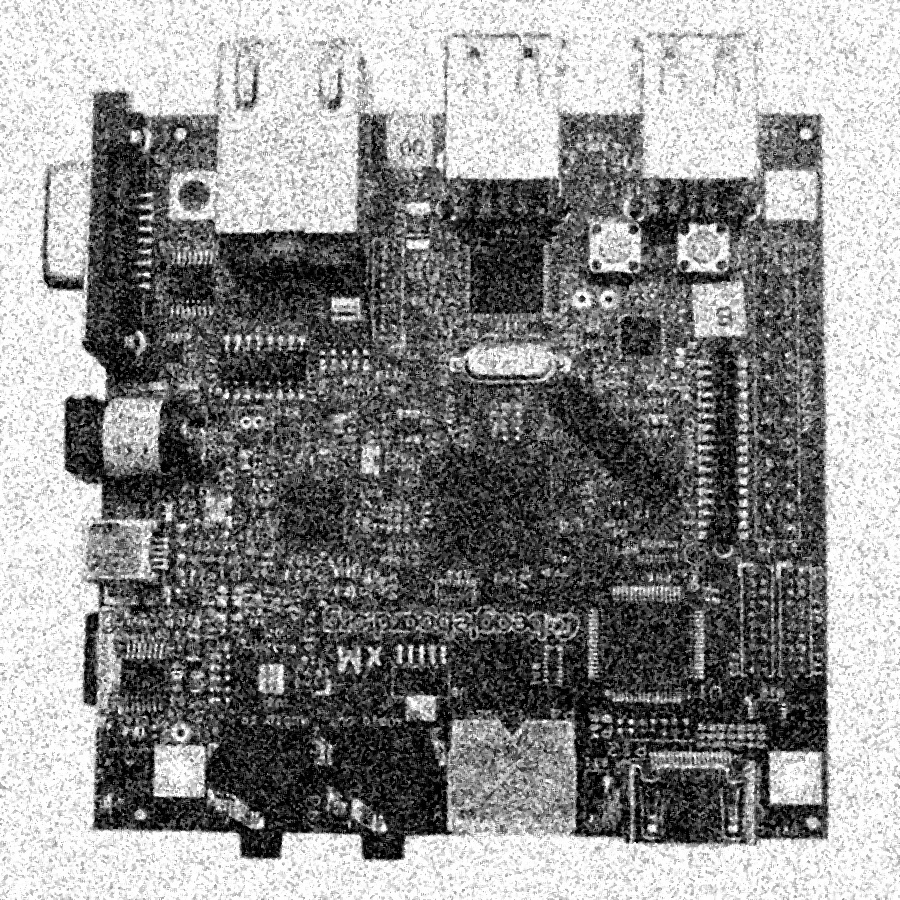
\includegraphics[height=7.5cm]{uniform-medianFilter.jpg}} 
\vspace{0.25cm}
\\ 
\small \textbf{ اعمال فیلتر میانگین } & \small \textbf{ اعمال فیلتر میانه } \vspace{0.5cm} \\ 

\end{tabular}}
\vspace{0.5cm}
\end{center} 


\subsection{سرعت اجرا}
\textbf{پرسش:}
سرعت اجرای کدام فیلتر بهتر است؟

\textbf{پاسخ:}
سرعت گاوسی و میانگین برابر و سرعت میانه به طرز چشم‌گیری تفاوت داشت. تفاوت نتیجه قابل قبول است (تصویر
 \lr{Full HD}
):

\begin{center}
\makebox[\textwidth]{%
\begin{tabular}{c}
\frame{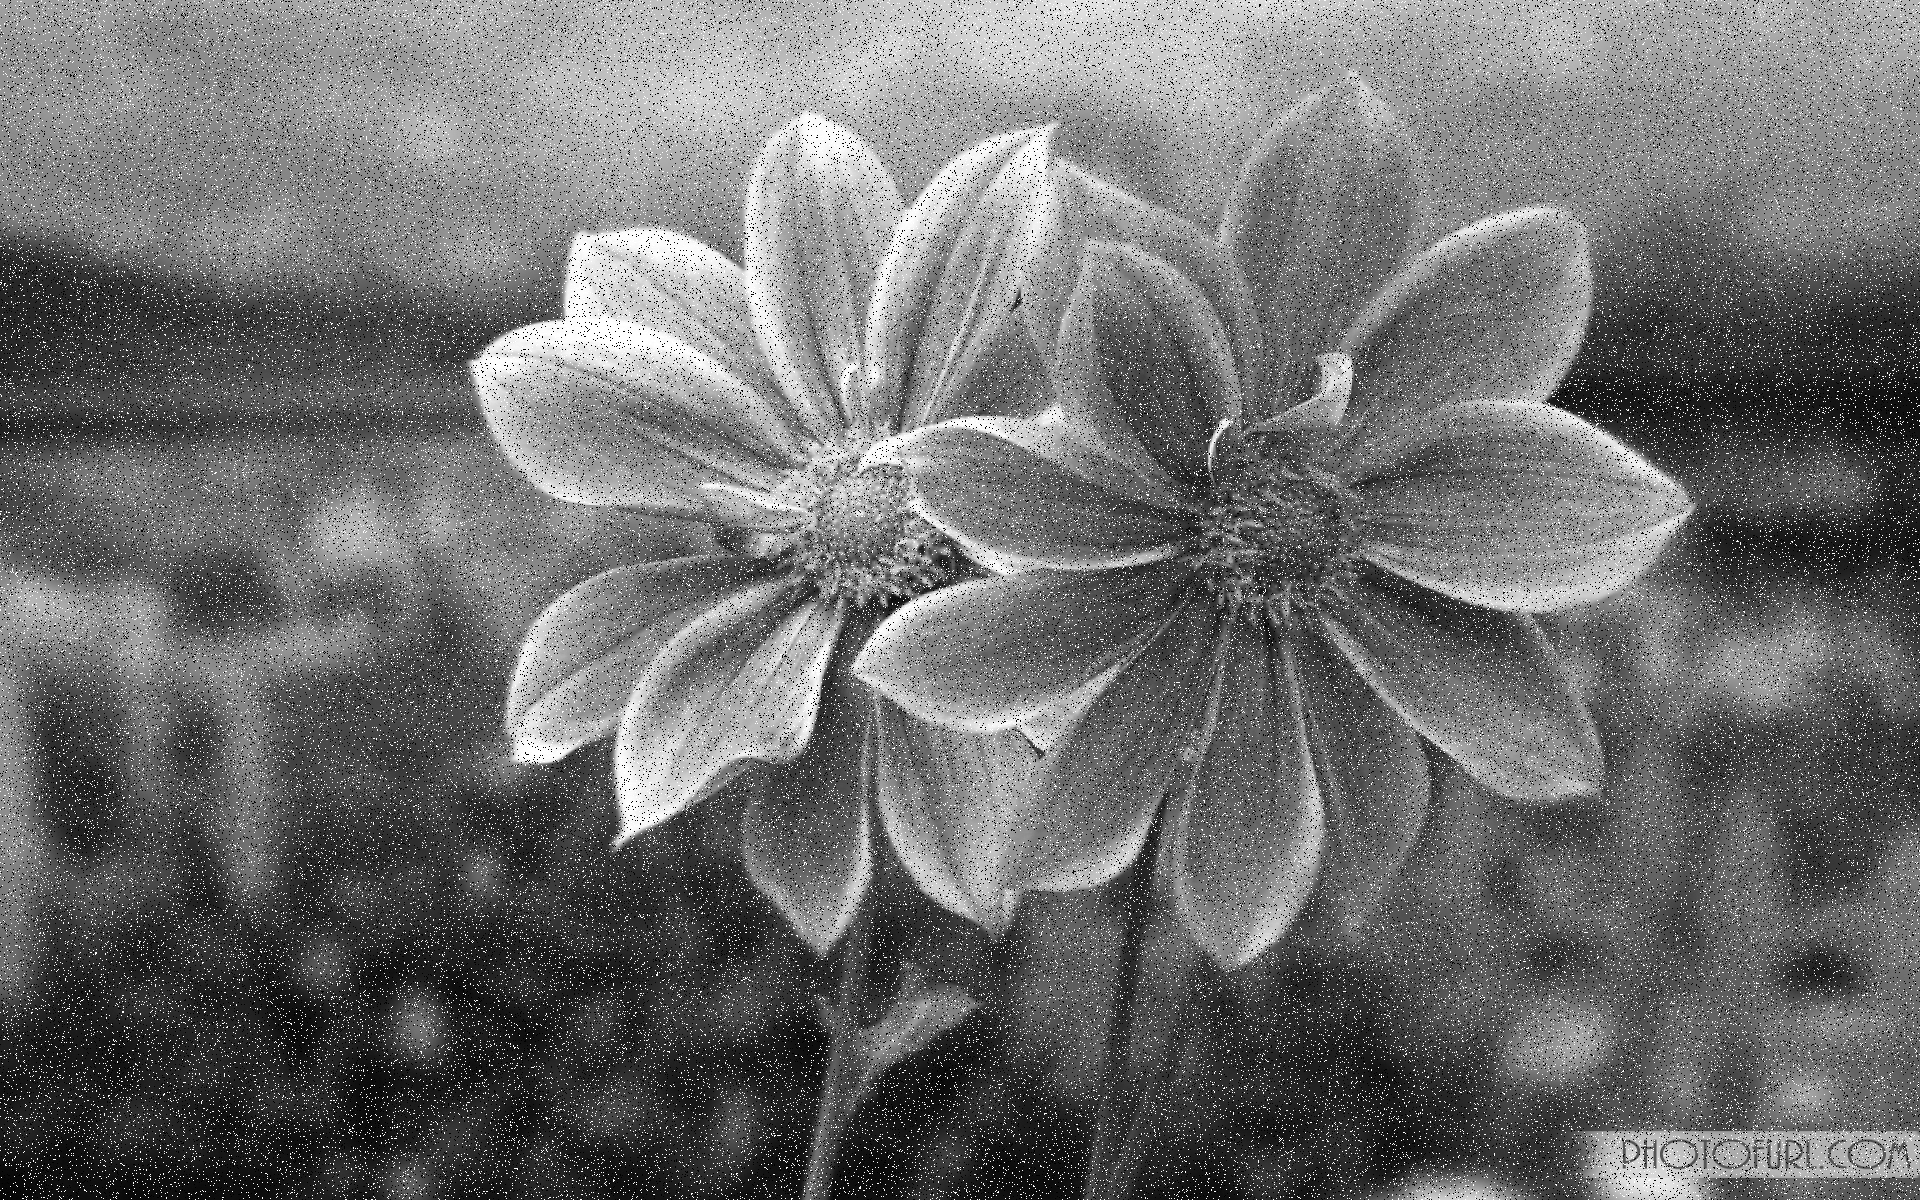
\includegraphics[height=7.5cm]{hd-sult.jpg}} \\
\small \textbf{ اعمال نویز نمک‌فلفلی } \\
\vspace{0.5cm} \\ 
\frame{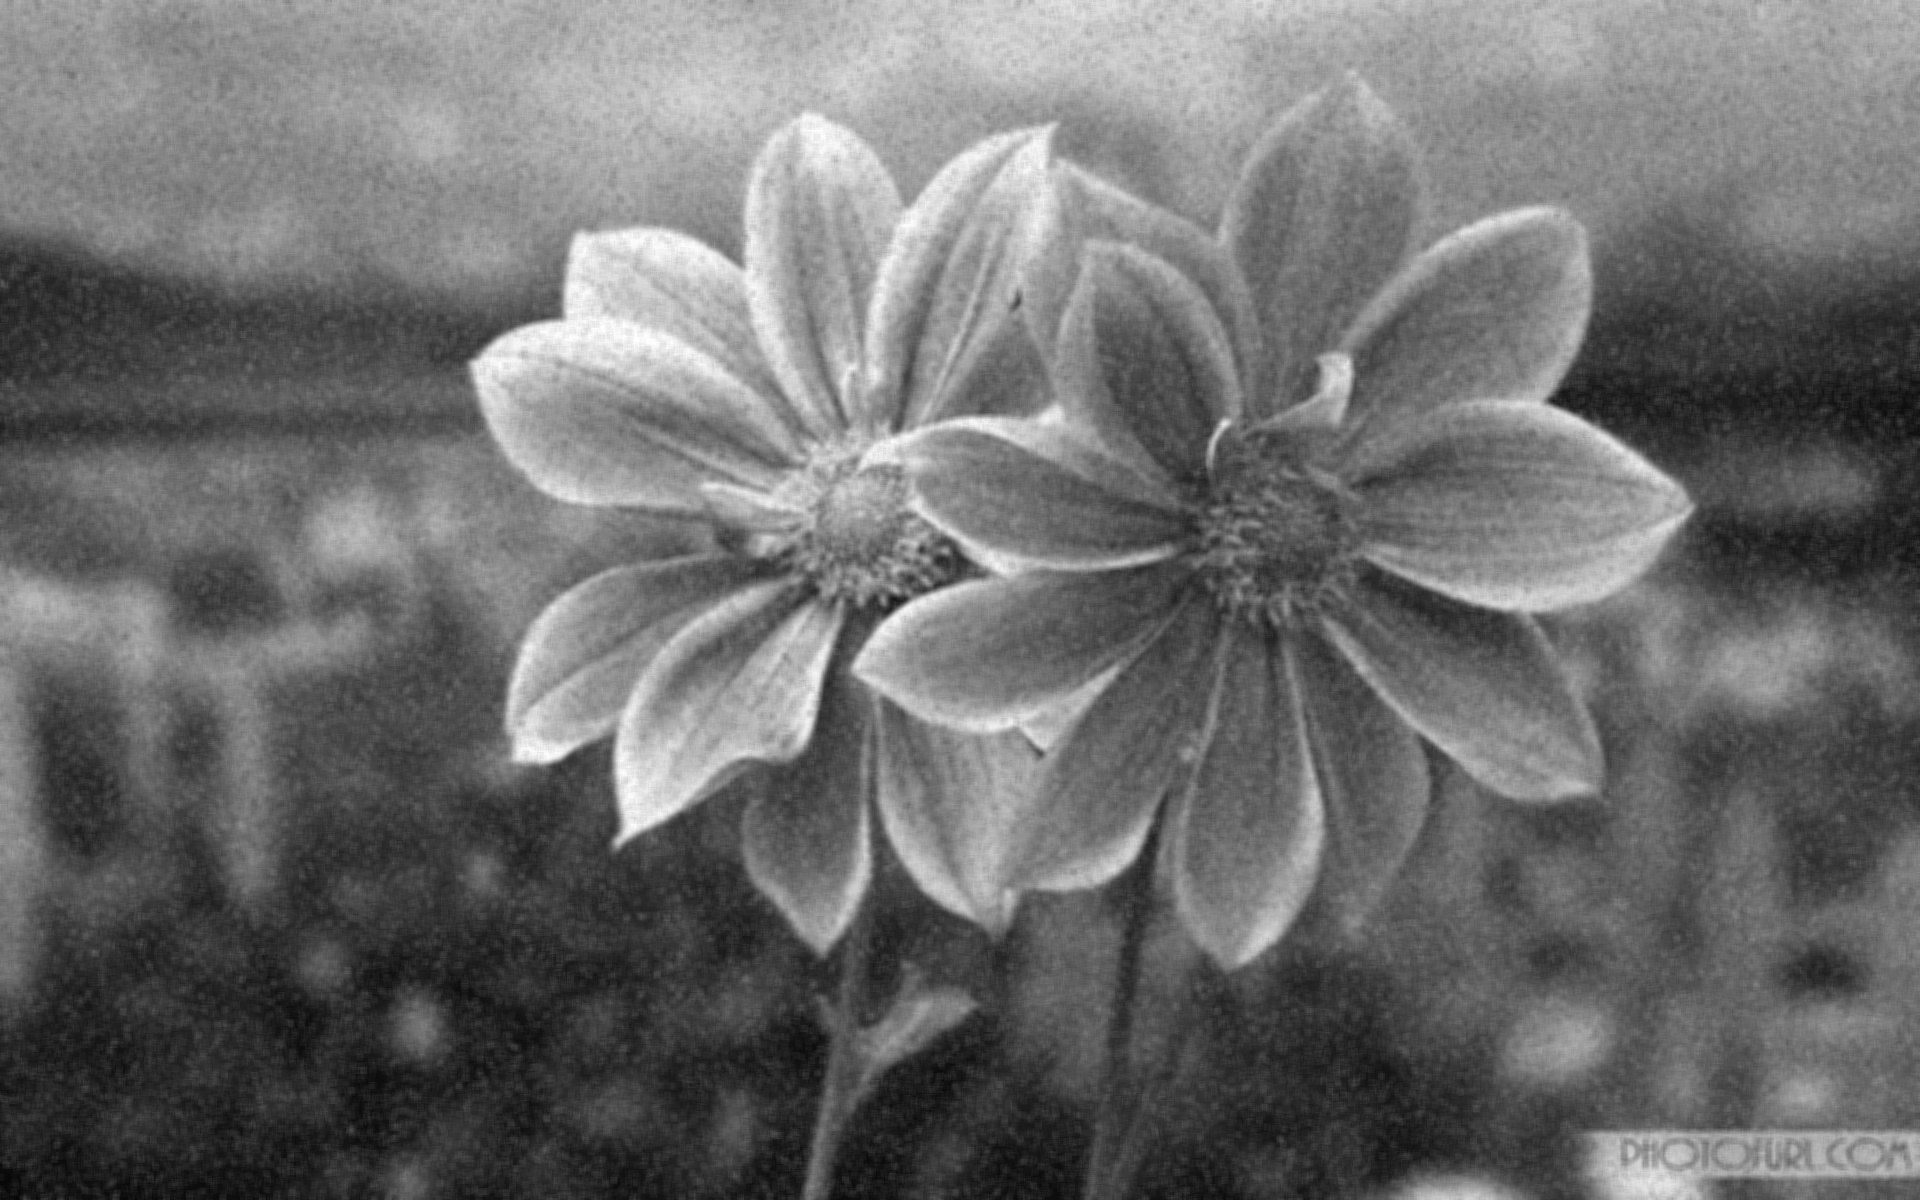
\includegraphics[height=7.5cm]{hd-meaqnFilter.jpg}} \vspace{0.25cm} \\ 

 \small \textbf{ اعمال فیلتر میانگین } \vspace{0.5cm} \\ 
 
\end{tabular}}
\vspace{0.5cm}
\end{center} 

 
\begin{center}
\makebox[\textwidth]{%
\begin{tabular}{c}
 
\frame{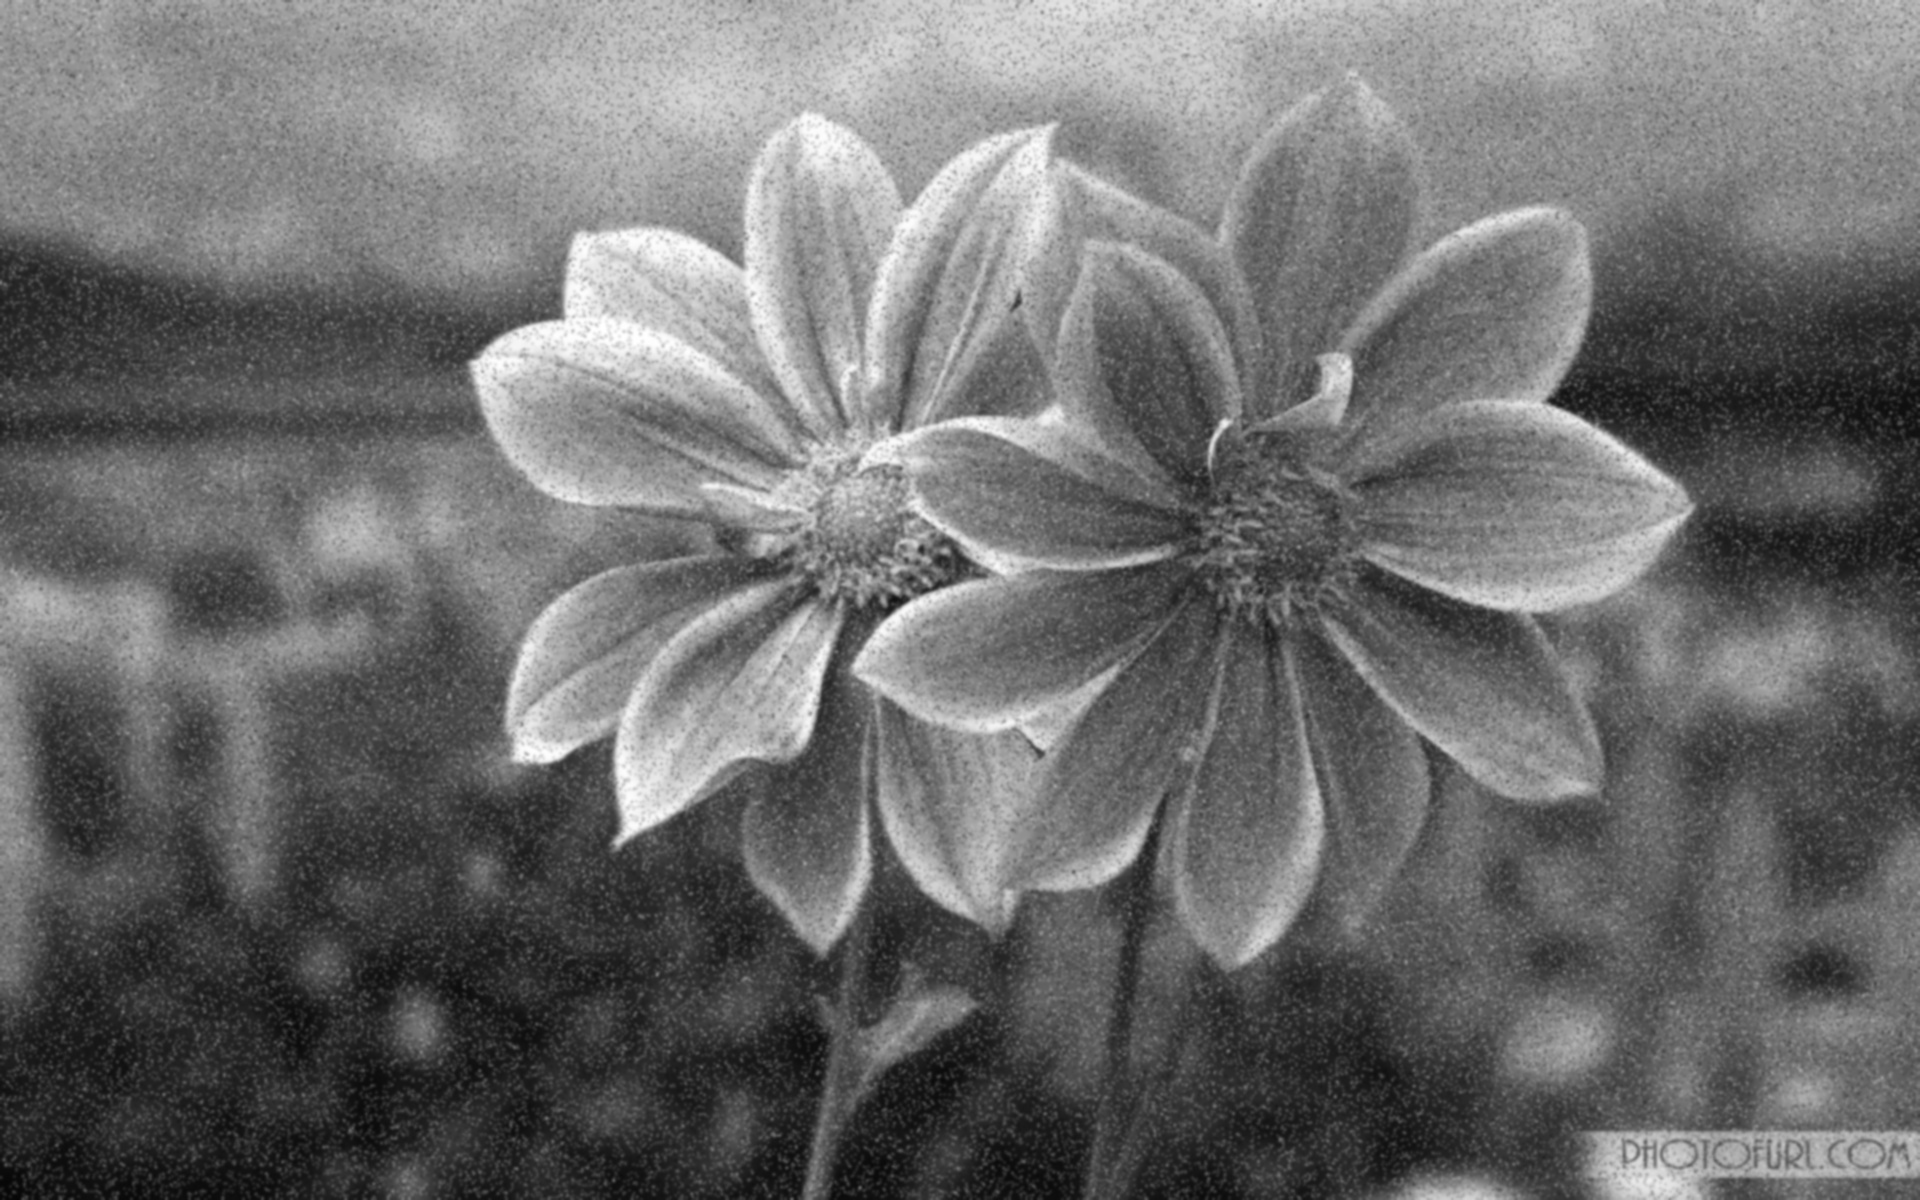
\includegraphics[height=7.5cm]{hd-gaussionFilter.jpg}} \\
\small \textbf{ اعمال فیلتر گاوسی } \vspace{0.5cm} \\ 
\frame{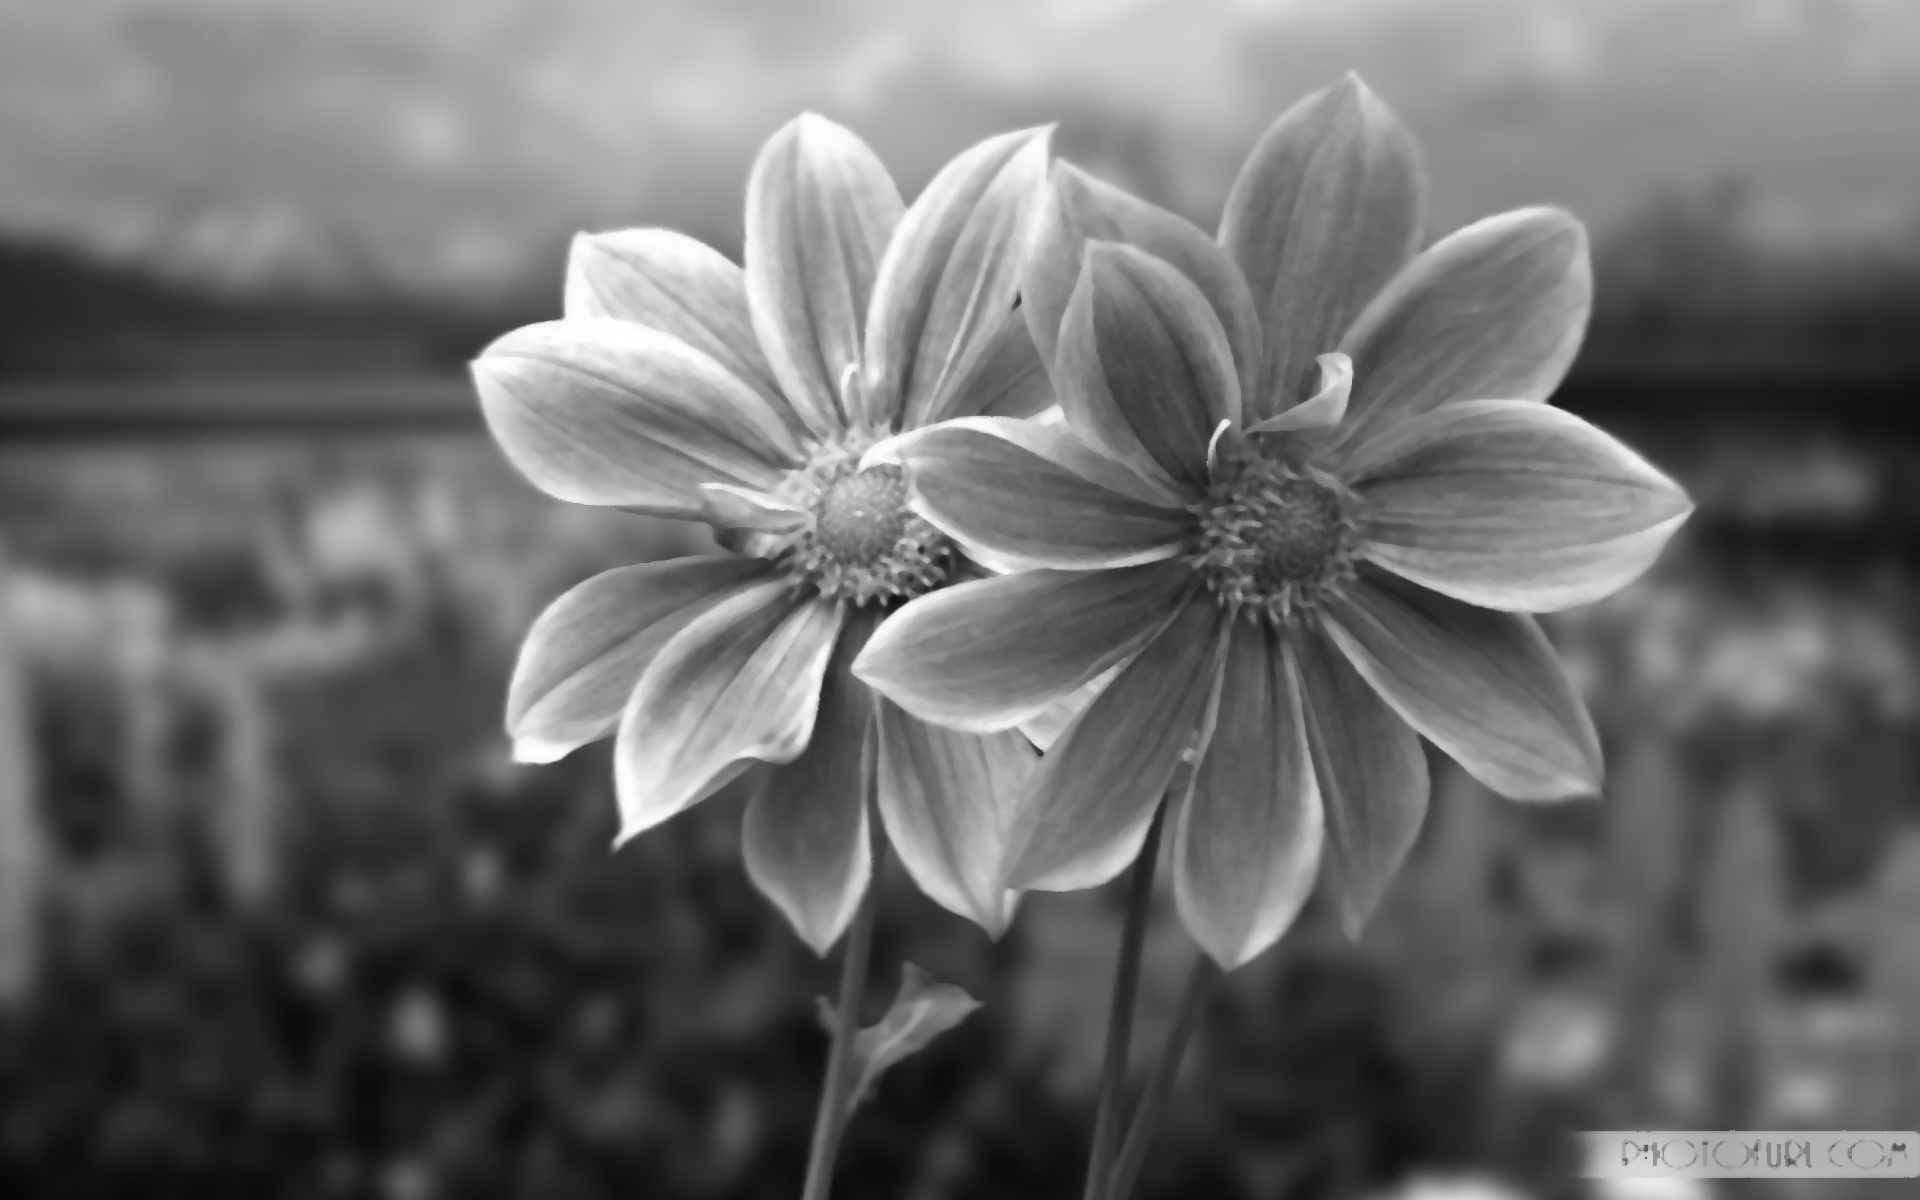
\includegraphics[height=7.5cm]{hd-medianFilter.jpg}} 
\vspace{0.25cm}
\\ 
\small \textbf{ اعمال فیلتر میانه } \\ 

\end{tabular}}
\end{center} 



\subsection{تاثیر اندازه پنجره}


\textbf{پرسش:}
اندازه پنجره فیلتر چه تاثیری دارد؟

\textbf{پاسخ:}
نتایج در ضمیمه‌ی گزارش آورده شده‌است. پنجره بزرگ‌تر در گاوسی و میانگین تصویر را مات‌تر می‌کند و در میانه باعث از بین رفتن برخی جزییات می‌شود.

%دستوری برای به حالت عادی درآمدن اندازه فونت‌ها 


\small
%ایجاد «مراجع»

\end{document} 
